% !TEX root = ../../prj4projektdokumentation.tex
% SKAL STÅ I TOPPEN AF ALLE FILER FOR AT MASTER-filen KOMPILERES 

\section{Intern blok diagram}
Herunder på figur \ref{fig:IBDSpaendingsregulator} ses et IBD for spændingsregulator. På diagrammet ses de interne forbindelser i systemet. Under figur \ref{fig:IBDSpaendingsregulator} er en signalbeskrivelse, der uddyber diagrammet.

\begin{figure}[htbp] % (alternativt [H])
	\centering
	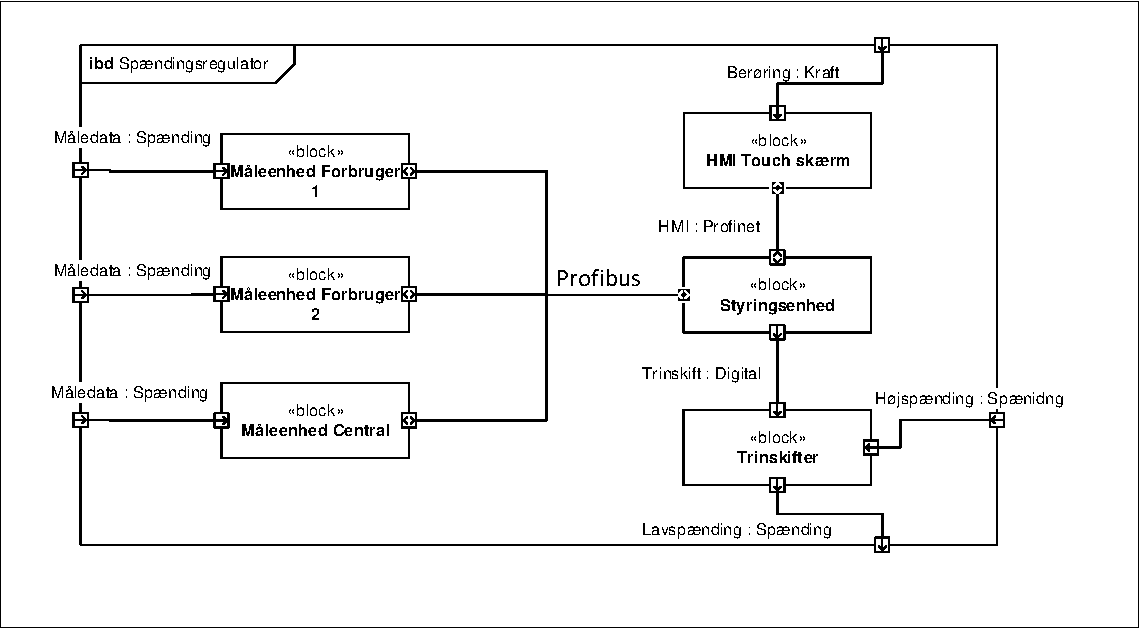
\includegraphics[width=0.8\textwidth]{Figure/IBDSpaendingsregulator}
	\caption{IBD Spændingsregulator}
	\label{fig:IBDSpaendingsregulator}
\end{figure}

\subsection{Signalbeskrivelse}

\begin{table}[ph]
	\centering
	\begin{tabular}{|p{2cm}|p{3cm}|p{2cm}|p{2cm}|p{4cm}|}
		\hline
		\textbf{Blok} & \textbf{Signal} & \textbf{Type} & \textbf{Signal-retning} & \textbf{Beskrivelse} \\\hline
		\multirow{2}{*}{Måleenhed} & Måledata & Spænding & In & Måledata er spændingingsniveauet på distributionslinjen. \\\hhline{~----} & Profibus & y & i & o \\\hline
		\multirow{2}{*}{HMI Touch skærm} & Berøring & Kraft & In & Berøring er en brugers interaktion med touch skærmen. \\\hhline{~----} & HMI & Profinet & Inout & Profinet er en tovejskommunikation med styringsenheden \\\hline
		\multirow{3}{*}{Styringsenhed} & HMI & Profinet & Inout & Profinet er en tovejskommunikation med HMI Touch skærm \\\hhline{~----} & Profibus & y & i & o \\\hhline{~----} & Trinskift & Digital & Out & Trinskift er en digital kommando til trinskifter om hvilket trin den skal vælge. \\\hline
		\multirow{3}{*}{trinskifter} & Trinskift & Digital & In & Trinskift er en digital kommando fra styringsenhed. \\\hhline{~----} & Højspænding & Spænding & In & Er spændingen på højspændingssiden af tranformeren. \\\hhline{~----} & Lavspænding & Spænding & Out & Er spændingen på lavspændingssiden af transformeren. \\\hline
	\end{tabular}
	\caption{Signalbeskrivelse}
	\label{tab:Signalbeskrivelse}
	
\end{table}

\newpage